\documentclass{beamer}

\usetheme{Warsaw}
\useoutertheme {miniframes}

\usepackage{xeCJK}
\setCJKmainfont{HanWangWCL06}

\begin{document}

\title[Linkit 7688 Duo Tutorial]{Linkit 7688 Duo Tutorial}

\author{Iblis Lin}

\date{2017/6/16}

\begin{frame}
  \titlepage
\end{frame}


\section{Big Picture}

\begin{frame}{Big Picture}
  \begin{center}
    \Huge
    把溫溼度 sensor data \\
    \uncover<2->{用 Linkit 讀出後,\\}
    \uncover<4->{透過網路,\\}
    \uncover<3->{塞進資料庫,\\}
    顯示在手機上
  \end{center}
\end{frame}


\section{Env setup}

\begin{frame}{Env setup}
  \begin{itemize}
    \item code \& slide: \url{https://github.com/APCLab/ict-iot}

    \item *Windows only* \url{https://support.apple.com/kb/DL999?viewlocale=en_US&locale=en_US}
  \end{itemize}
\end{frame}

\begin{frame}{Config Arduino IDE}
  Arduino 安裝 Linkit 的 Plugin

  > Perference

  \url{http://download.labs.mediatek.com/package_mtk_linkit_smart_7688_test_index.json}
\end{frame}

\begin{frame}[fragile]{Config Linkit}
  \Large
  \begin{itemize}
    \item 預設 Linkit 會作為一個 AP,可共連線

    \item 第一次 login 時,使用 \verb|mylinkit.local| 連線

    \item 先改密碼!
  \end{itemize}
\end{frame}

\begin{frame}[fragile]{Config Linkit Hostname}
  \Large
  \begin{center}
    改一下 hostname,避免大家用相同的
  \end{center}

  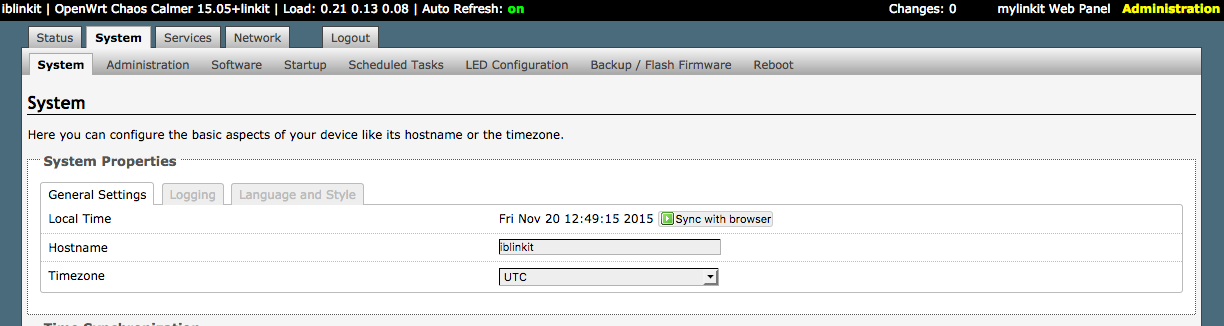
\includegraphics[scale=0.25]{./img/hostname.png}

  \begin{center}
    我的是 \verb`iblinkit`

    之後使用 \verb`iblinkit.local` 連線
  \end{center}
\end{frame}

\begin{frame}{Config Linkit Network}
  \Large
  \begin{center}
    最後回來改掉 AP mode

    換成 station mode 以連上其他 wifi AP
    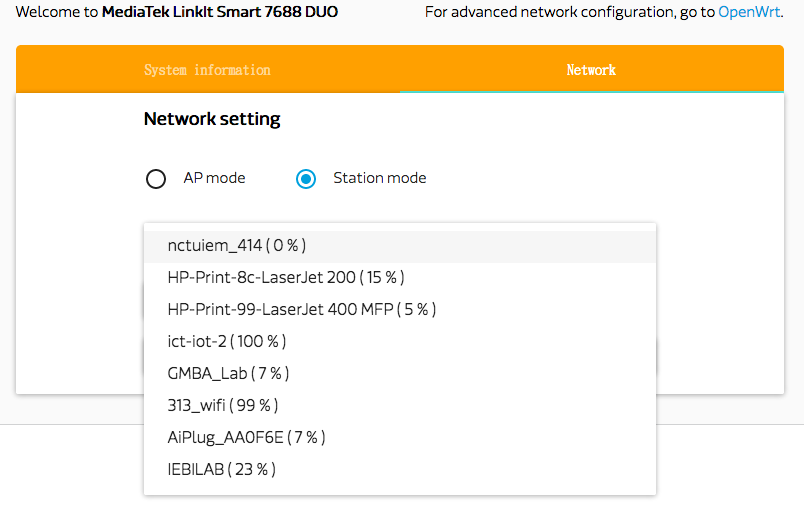
\includegraphics[scale=0.3]{./img/connect_wifi.png}
  \end{center}
\end{frame}

\section{Linkit}

\begin{frame}
  \begin{center}
    \Huge
    Linkit 讀取 sensor data
  \end{center}
\end{frame}

\begin{frame}[fragile]{Burn code}
  \Huge
  copy out the folder \verb|linkit-7688-duo/dht22|
\end{frame}


\section{appmate}

\begin{frame}{appmate overview}
  \Large

  \begin{itemize}
    \item 簡單的 Web application

    \item Django project

    \item 所以是使用 Python

    \item 提供 與 database 互動的 http API

    \item API 採用 REST design

    \item 我們把它設計成 template project
  \end{itemize}
\end{frame}

\begin{frame}[fragile]{appmate setup}

  建立 database, 這裡預設是使用 SQLite
  \begin{block}{code}
  \begin{verbatim}
    python ./maange.py migrate
  \end{verbatim}
  \end{block}

  建立 Django 後臺的 admin user
  \begin{block}{code}
  \begin{verbatim}
    python ./manage.py createsuperuser
  \end{verbatim}
  \end{block}
\end{frame}

\begin{frame}[fragile]{appmate setup}
  Run the server!
  \begin{block}{code}
  \begin{verbatim}
    python ./manage.py runserver
  \end{verbatim}
  \end{block}

  並且仔細看看畫面上的訊息
\end{frame}

\begin{frame}{appmate}
  \begin{itemize}
    \item check \url{http://tz.firc.tw:4000/}

    \item check \url{http://tz.firc.tw:4000/major/}
  \end{itemize}
\end{frame}

\end{document}
